
\chapter{Implementation of CVLiBG mobile library}
This chapter describes the implementation of a mobile library for computer vision enhanced applications on Android devices. An abstract example of such an application may look like this:

\begin{figure}[hbt]
	\centering
	\includegraphics[width=0.7\textwidth]{obrazky-figures/final_result_scheme.pdf}
	\caption{Result application detecting cards for a card game Bang!}
	\label{ResultApplicationScreenshot}
\end{figure}

The figure above shows a mobile application detecting game objects, in this case, cards from the game Bang!. The application provides additional information and tips not drawn onto the card. This may allow players to skip reading the game manual or use it as a quick reminder, especially for cards with a large number of unique cards. Use of the mobile library for this specific game is described in chapter \ref{bangImplementation}.

The goal of this library is to provide an easy to use solution for creating mobile applications using object detection with the on device camera to detect game objects. This library should help with developing final applications, prototypes, and proof-of-concept applications. All of the above mentioned goals are achieved while giving developers a modular interface and not limiting them in other aspects of application development. 

% ===========================================================================================

% ===========================================================================================


\section{Android development with Kotlin}
This section explores the choices made during the selection of the operating system and environment used for developing the library. The general knowledge about Android and Kotlin was mostly gained from the Kotlin documentation \cite{kotlinDocs}, the Android API documentation \cite{androidDocs}, and ARM's online course \cite{armTutorial} alongside the YouTube version of the same course \cite{armYtTutorial} for Android application development using the OpenCV camera, which was used as a starting point.

\subsection{Operating system}
Operating systems for mobile phones are mostly dominated by two systems: Android and iOS. Since 2020, the smartphone market share has been steadily at 70\% \cite{phoneOsStatistics} in favor of Android over iOS. For this reason, Android was chosen as the target operating system.

\subsection{Programming language and integrated development environment}
For a long time, Java was the main programming language for Android development. However, in 2019 \footnote{Android's Kotlin first approach: \url{https://developer.android.com/kotlin/first}}, Google announced the introduction of the Kotlin language. The blog also highlights Kotlin's advantages, such as its easier to understand code, safer null exception handling, and exceptional concurrency handling. One of the biggest advantages of the Kotlin language is its interoperability with Java. This feature is crucial, as it allows Kotlin code to use Java code and vise versa, which means that using Kotlin results in less code overhead while keeping all the benefits and support of the Java packages created over the long duration of Java's existence. For this reason, Kotlin was chosen as the main programming language.

The most popular integrated development environments (hereafter referred to as IDEs) for developing applications in Android are Android Studio and IntelliJ Idea. Both IDEs are similar at first glance, as they also share internal code \footnote{JetBrains blog post on IntelliJ Idea and Android studio: \url{https://blog.jetbrains.com/idea/2013/05/intellij-idea-and-android-studio-faq/}}. While the recommended approach for Android development is to use Android Studio, I, as the author, leaned toward IntelliJ Idea due to  personal preference and previous experience.

\subsection{OpenCV}
OpenCV \footnote{OpenCV's about page: \url{https://opencv.org/about/}} is a multi-platform and multi-language open source library with algorithms for computer vision, machine learning, image manipulation, and many more use-cases. It is a well established library used by many companies and institutions, such as NASA, ARM, JetBrains, and others. One of the main advantages of OpenCV is its near native speed performance with precompiled C++ code.

This thesis utilizes OpenCV for its excellent support of computer vision algorithms utilized by both CVLiBG and Dataset Creator. The library is used for image manipulation tasks, such as resizing, normalizing, letterboxing, and more computer vision based tasks, such as Non-maximum Suppression for filtering duplicate detections. OpenCV also supports performing inference runs for CNN based neural networks; however, this use-case was mostly replaced.

% ===========================================================================================

% ===========================================================================================

\section{Android application}
Android applications are mostly composed of Android's \texttt{Activity} \footnote{Android API: Activity: \url{https://developer.android.com/reference/android/app/Activity}} classes, which contain the code and behavior of a given activity, and layouts describing the positions, sizes, and padding of user interface (hereafter referred to as UI) related elements. 

Activities are meant to contain code related to UI elements. They also serve as a separation for task specific parts of the applications, such as home, settings, search, etc. Activities are also used as navigation points. CVLiBG does not interfere with this, nor does it provide any help with managing or navigating the activities. It should be noted that the first activity to launch or to use the camera should ask for permission to use it. This can be achieved either manually or by using the \texttt{CommonUtils.checkCameraPermission()} static method.

% ===========================================================================================

% ===========================================================================================

\subsection{Android Manifest}
The \texttt{AndroidManifest.xml} file contains project specific information and must be placed in the project's root folder. All projects using CVLiBG require camera permission \footnote{Android manifest, permissions: \url{https://developer.android.com/guide/topics/manifest/manifest-intro\#perms}}:



\label{androidManifestExample}
\begin{lstlisting}
<?xml version="1.0" encoding="utf-8"?>
<manifest xmlns:android = "http://schemas.android.com/apk/res/android">
    <uses-permission android:name = "android.permission.CAMERA"/>
        ...
</manifest>
\end{lstlisting}

% ===========================================================================================

% ===========================================================================================


\subsection{Concurrency and Coroutines}
\label{concurrencyExplained}
One of Kotlin's key features is its concurrency handling, achieved with relatively low code overhead. Kotlin allows developers to write asynchronous code in a sequential style. This language feature abstracts away much of the complexity associated with thread management \cite{kotlinConcurrency}.

Non-blocking context switching is achieved with the \texttt{withContext} function, which allows the code inside a coroutine to switch to different contexts while maintaining the sequential code style. Coroutines use dispatchers, which schedule execution threads or a pool of threads. The most commonly used dispatchers are \texttt{Main}, \texttt{IO}, and \texttt{Default}. The \texttt{Main} dispatcher is used for executing code on the main thread, which also manages the UI. Usually, manipulating UI elements outside of the main thread results in a runtime exception. The \texttt{Default} thread pool is used for CPU-heavy computations, such as the benchmarks described later that can take a few minutes to complete. The last dispatcher is for input and output operations.

Kotlin also allows developers to group coroutines using a principle called structured concurrency. This principle treats coroutines as a hierarchical tree of parent and child tasks. These so-called scopes allow coroutines to define lifecycle boundaries and manage coroutines within the scope \cite{kotlinConcurrency}.

\begin{minipage}{\textwidth}
\begin{verbatim}
fun foo() {
    lifecycleScope.launch {
        withContext(Dispatchers.Main) {
            updateText()
            updateColor()
        }

        withContext(Dispatchers.IO) {
            writeToStorage(text)
            writeSendOverHTTPS(text)
        }
    }

    Log.d("foo()", "foo() finished")
}
\end{verbatim}
\end{minipage}
\bigskip


The code above shows the function \texttt{foo()}. This function is not a suspend function and can be called synchronously. Within the function, a new coroutine is launched using the current context from which \texttt{foo()} is called. First, \textbf{updateText()} and \textbf{updateColor()} will be executed in the main dispatcher. This essentially allows \texttt{foo()} to manipulate UI elements even if run on another thread. After both of these methods finish, one after another, the context will be switched to the \texttt{IO} dispatcher, and long operations will be executed. All of this code would be finished on the launched coroutine while the \texttt{foo()} method would finish almost instantly after printing the log.



% ===========================================================================================

% ===========================================================================================
 
\section{Camera Controller}
\label{CameraController}

The \texttt{CameraController} class is responsible for managing the camera and initializing the analysis of the image data from the camera. Internally the controller uses Android's \texttt{CameraX} \footnote{CameraX overview: \url{https://developer.android.com/media/camera/camerax}} and \texttt{CameraProvider} \footnote{CameraProvider API reference: \url{https://developer.android.com/reference/androidx/camera/lifecycle/ProcessCameraProvider}}, which is a modern solution for capturing and analyzing images from the smartphone's camera. 
The \texttt{CameraProvider} is set up with two use cases: image preview using \texttt{PreviewView} \footnote{Android Preview: \url{https://developer.android.com/reference/androidx/camera/core/Preview}} \footnote{Android PreviewView: \url{https://developer.android.com/reference/androidx/camera/view/PreviewView}} and image analysis using \texttt{ImageAnalysis} \footnote{Android Image Analysis: \url{https://developer.android.com/reference/androidx/camera/core/ImageAnalysis}}.

The image analysis uses \texttt{ImageAnalyzer} and \texttt{Detector} classes as a modular solution for object detection (see \ref{Detector}). Furthermore, to keep the UI responsive, the image analysis is using the \texttt{ExecutorService} \footnote{\url{https://developer.android.com/reference/java/util/concurrent/ExecutorService}} to execute the analysis on another thread. 

It also uses the \texttt{ImageAnalysis.STRATEGY\_KEEP\_ONLY\_LATEST} to keep and analyze only the latest images. While this means that some data are lost, it results in a responsive camera preview while detections and images are being processed as fast as possible.





The \texttt{CameraProvider} is bound to the \texttt{Lifecycle} \footnote{Activity lifecycle: \url{https://developer.android.com/guide/components/activities/activity-lifecycle}}, which automatically manages the transition from one activity to another or mobile rotations by recreating the fragment without memory leaks. The executor and other variables used by \texttt{ImageAnalyzer} or \texttt{Detector} classes must be cleaned up; otherwise, a memory leak or errors might occur. This can be done manually by calling the \texttt{stop()} method or setting \texttt{bindToLifecycle=true} during the initialization of the controller, which will handle the cleanup automatically. 

\subsection{Initializing the Camera Controller}
The \texttt{CameraController} requires UI elements, two \texttt{Detector} classes, and \texttt{LifecycleOwner}. 

The UI elements are used for the camera preview and for displaying the results of object detection. By default, the \texttt{PreviewView's} scaling type is set to \texttt{FILL\_CENTER}. This option scales the preview to the screen while keeping the aspect ratio, cropping one of the dimensions (width or height) to fit the screen. This approach is recommended; other approaches might require changing the \texttt{DetectionOverlay} implementation (see \ref{DetectionOverlay}).

One of the detectors is used for realtime detection running on top of the camera preview, and the detailed detection, which freezes the image and waits for \texttt{the Detector} to finish image analysis. \texttt{CameraController} builds detectors once the \texttt{start()} method is called; this enables unused camera controllers and detectors to have a smaller memory footprint. The \texttt{start()} method is a suspend function, and it is required to launch it in a coroutine using the main dispatcher's context. 

The \texttt{lifecycleOwner} is used for binding the \texttt{CameraController}. If this option is enabled, the controller will be destroyed and freed automatically upon changes in activity, rotation, or closing the application. This option is enabled by default.

\begin{itemize}
    \item context -- \texttt{Context} -- used for loading \texttt{Detectors} from assets
    \item lifecycleOwner -- \texttt{LifecycleOwner}
    \item previewView -- \texttt{androidx.camera.view.PreviewView}
    \item detectionOverlay -- \texttt{DetectionOverlay}
    \item metricsOverlay -- \texttt{MetricsOverlay?} -- optional on-screen metrics for debugging
    \item realtimeDetector -- \texttt{Detector?}
    \item qualityDetector -- \texttt{Detector?}
    \item bindToLifecycle -- \texttt{Boolean} -- default value is true
    \item previewViewScale -- \texttt{PreviewView.ScaleType}
\end{itemize}

\subsection{Required UI layout}
\label{CameraFragmentOverlays}
The fragment containing the \texttt{CameraController} is required to place the preview and overlays on top of each other with the same size in order for detections to be visible on top of the \texttt{previewView}.

\begin{figure}[hbt]
	\centering
	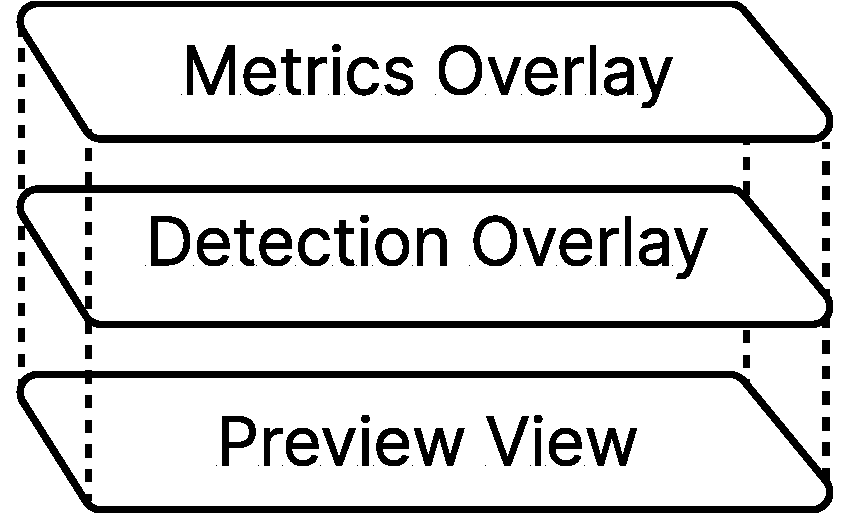
\includegraphics[width=0.4\textwidth]{obrazky-figures/camera_fragment_overlay.pdf}
	\caption[Camera preview, detection overlay, metrics layout]{Layout of user interface elements required by the \texttt{CameraController} where detections are on top of the preview of the camera.}
\end{figure}

\subsection{Choosing resolution and the aspect ratio of the camera}

The \texttt{ImageAnalyzer} and the \texttt{PreviewView} \footnote{Camera Preview: \url{https://developer.android.com/media/camera/camera2/camera-preview}} require the resolution at which they will operate. The resolution is determined by the detectors. Higher pixel count (\texttt{width x height}) is used as the base for finding the resolution. If the camera cannot provide the resolution \cite{androidCameraResolution}, it will use a
\begin{lstlisting}
    ResolutionStrategy.FALLBACK_RULE_CLOSEST_HIGHER_THEN_LOWER
\end{lstlisting}
which will choose the closest resolution higher than the specified one. This achieves the lowest possible resolution, which speeds up the preprocessing of the images while losing as little detail as possible.

Object detection models, such as YOLO, which are used in this project, usually expect a \texttt{640x640} screen resolution with a \texttt{1:1} aspect ratio. However, not all devices support this, or they would have to rescale the image, causing performance decreases. Furthermore, the preview will be displayed onto mobile screens, which usually do not use the \texttt{1:1} aspect ratio. Based on the statistics \cite{aspectRatioStats}, the most common, or rather the closest to it, is \texttt{16:9}. Other supported options, such as \texttt{4:3} , would likely waste performance as the excess will be cropped from the screen.


% =========================================================================================

% =========================================================================================


\section{Image Analyzer}
The \texttt{ImageAnalyzer} uses camera images as input and outputs analyzed images. It implements CameraX's \texttt{ImageAnalysis.Analyzer} \footnote{Android's API reference: ImageAnalysis \url{https://developer.android.com/reference/androidx/camera/core/ImageAnalysis}} interface and its \texttt{analyze()} method, with \texttt{ImageProxy} as its input. The \texttt{ImageProxy} class contains information about the input image from the camera.

To analyze images, it uses two detectors derived from the abstract \texttt{Detector} class. These detectors work as simple modules, detecting objects from an input bitmap and outputting results of these operations. Furthermore, \texttt{ImageAnalyzer} contains logic for switching between two operating modes, each using a different detector. 

\textbf{Realtime} mode analyzes input data as fast as possible. This mode does not synchronize with the camera preview, which means that the projected outputs are always from the "past". Therefore, it is recommended to use lightweight models with small latency for the \texttt{realtimeDetector} used in this mode.

On the other hand, the \textbf{detailed} mode will, upon activation, analyze the first image, pause image analysis, and output the image analysis alongside the input image. Therefore, instead of analyzing camera inputs as fast as possible, it analyzes a single image, like a photo. This mode uses \texttt{detailedDetector} provided to \texttt{ImageAnalyzer} in its constructor.

Switching between the two modes can be achieved with \texttt{switchToDetailedAnalysis()} and \texttt{switchToFasterAnalysis()} methods, or similarly named methods from the camera controller.

\subsection{Collecting detector results}
\texttt{ImageAnalyzer} utilizes Kotlin's \texttt{Flow} functionality, specifically, it uses \texttt{StateFlow} \footnote{Kotlin flows on Android: \url{https://developer.android.com/kotlin/flow}} \footnote{StateFlow Android Guide: \url{https://developer.android.com/kotlin/flow/stateflow-and-sharedflow}}. Unlike simpler approaches like callback functions, this approach allows multiple data consumers across different threads while maintaining thread safety. \texttt{ImageAnalyzer} exposes \texttt{detectionResult} , containing results of image analysis, and \texttt{metrics} , containing performance and additional metrics. Metrics can be enabled with \texttt{setMetricsEnabled()} and \texttt{setVerboseMetricsEnabled()} methods, or using likewise named methods from the \texttt{CameraController}.

When using this data inside UI fragments or activities, it is required to use lifecycle aware code that resets when the view is being destroyed; otherwise, this behavior may lead to application crashes. Example of safe use inside an activity or fragment:

\begin{verbatim}
    viewLifecycleOwner.lifecycleScope.launch {
        viewLifecycleOwner.repeatOnLifecycle(Lifecycle.State.STARTED) {
            viewModel.imageAnalyzer?.detectionResult?.collect {
                binding.detectionOverlay.update(it)
            }
        }
    }
\end{verbatim}

% ===========================================================================================

% ===========================================================================================


\section{Detector}
\label{Detector}
The abstract \texttt{Detector} class is an interface-like solution for unifying object detection algorithms. Its main functionality is the public method \texttt{run(bitmap)}, where bitmap is an input image.

It should be noted that the \texttt{Detector} created with its constructor is not ready to use and requires the \texttt{build()} method to be called before use. This function returns a \texttt{DetectionResult} object, containing a list of detections. \texttt{Detector} can be constructed using these common parameters:

\bigskip
\begin{itemize}
  \item {modelPath -- path to the model inside the assets folder}
  \item {confThreshold -- threshold value used for filtering detection}
  \item {applyNMS -- whenever Non-Maximum Suppression should be applied}
  \item {nmsThreshold -- Intersection over Union threshold for NMS}
  \item {inputDataSize -- expected size of images used by the model}
\end{itemize}
\bigskip

Furthermore, as an abstract class, \texttt{Detector} requires developers to implement these methods:

\bigskip
\begin{itemize}
  \item {\texttt{detect(image: Bitmap) : DetectorResult} -- method defining the object detection process. Input of this method is bitmap and returns \texttt{DetectionResult} containing list of detection, metrics, and usefull information (see \ref{DetectorResult}).}
  \item {\texttt{runtimeSetup(assetService: AssetService)} -- method called before the detect method. This should be used for setting up the runtime, loading model and other necessaries for given detection task. The \texttt{AssertService} can be used for loading models as a ByteArrays from the assets folder.}
  \item {\texttt{destroy()} -- optional cleanup for allocated memory called afther the \texttt{ImageAnalyzer} and \texttt{Detector} are destroyed .}
\end{itemize}
\bigskip

\subsection{Ready-to-use and abstract Detectors}
As mentioned before, this library uses OpenCV's image manipulation algorithms. OpenCV also contains the \texttt{DNN} package, which can be used as an inference runtime. This approach, however, was replaced by ONNX's Runtime, which, based on testing, provides almost 2 times faster inference. 

The key idea of CVLiBG is to be modular and reusable. However, it should not force developers into loading unwanted modules, should they decide not to use them. Because of that, ONNX's implementation of detectors was separated into another module. This enables developers to use CVLiBG and implement their own detectors or use OpenCV's predefined implementation without the need for an additional library that might not be utilized. The list of predefined detectors from both modules:

\begin{itemize}
  \item {\texttt{AbstractYoloDetector} is an abstract class containing common methods and algorithms for all YOLO-based detectors.}
  \item{\texttt{YoloOpenCV} uses OpenCVs \texttt{Dnn} inference engine. It supports YOLO version from 8 to 11 and extends the \texttt{AbstractYoloDetector}.}
  \item {\texttt{YoloOnnxDetector} is based on \texttt{AbstractYoloDetector} and is usable for YOLO models from version 8 to version 11. The detector uses the ONNX runtime as an inference engine.}
  \item {Yolo26OnnxDetector is a specialized version of \texttt{YoloOnnxDetector} for YOLO26 version.}
\end{itemize}
\bigskip

All of the above mentioned \texttt{Detectors} implement scaling of the \texttt{Detection} objects back to the original bitmap resolution. This, however, is not mandatory and depends on the developers. Should the developers choose to implement this scaling in other parts of the application, it can be done using the \texttt{ImageDetails} data class, which is part of \texttt{DetectionResult}. \texttt{DetectionOverlay} already contains these details as they are provided to it alongside the list of detections. An example code utilizing \texttt{imageDetails} to scale detections to input image size:

\begin{verbatim}
    scaledX = (x - imageDetails.padX) / imageDetails.scale
    scaledY = (y - imageDetails.padY) / imageDetails.scale
    scaledW = width / imageDetails.scale
    scaledH = height / imageDetails.scale
\end{verbatim}


% ===========================================================================================

% ===========================================================================================

\subsection{Detector Registry}
\label{DetectorRegistry}
Most applications might use one or two detectors. However, some applications might utilize switching between models and detectors. This is mostly due to the fact that a single implementation of the \texttt{Detector} class can handle different models as long as their inputs and expected outputs match. For example, the \texttt{YoloOnnxDetector} supports any YOLO model from version 8 to 11 of any size in ONNX format. This also allows the use of different detectors with different models, which are interchangeable during the runtime of the application. 

However, this also introduces a problem where detectors might be used with incompatible models. The \texttt{DetectorRegistry} is meant to solve this problem. It provides a way for developers to register the models from the project assets with the correct detector. This way, an incompatible model will not be paired with an incompatible \texttt{Detector}. This is mostly possible because the \texttt{Detector} objects do not load the models on initialization, but only after \texttt{the build()} method, leaving the registry's memory usage low.

\begin{lstlisting}
    DetectorRegistry.register("Register key", "model_path.model_extension")
            { path -> YoloOnnxDetector(path, applyNMS = false) }
\end{lstlisting}
Retrieving the \texttt{Detectors} can be achieved with:
\begin{lstlisting}
    DetectorRegistry.createDetector("Register key")
\end{lstlisting}

The registration process requires a string key and a path to the model, which is located in the assets directory under the \textit{models/} directory. The last part is a lambda function for creating an instance of the \texttt{Detector} class. The \texttt{DetectorDerivedClass} is the name of the class inheriting from the \texttt{Detector} abstract class. Some of the detectors have different optional parameters, which can be specified in the lambda function, such as the use of Non-Maximum suppression or a threshold for detection filtering. 

% ===========================================================================================

% ===========================================================================================

\section{DetectionOverlay}
\label{DetectionOverlay}

The \texttt{DetectionOverlay} is an open class used for drawing detections on top of the camera preview (\ref{CameraFragmentOverlays}). This class contains a default implementation of the \texttt{drawDetections()} method; however, it is strongly recommended to subclass \texttt{DetectionOverlay} and rewrite this method to suit the application's style, theme, and information level provided to users. 

The \texttt{ImageAnalyzer} updates the information needed by the \texttt{DetectionOverlay} after the active \texttt{Detector} has finished analyzing the image. Furthermore, it supports drawing the entire background image. This feature is mainly used when the \texttt{ImageAnalyzer} is switched to detailed mode with \texttt{switchToDetailedAnalysis()} method. Therefore, the image is "frozen", and slower, more detailed detections are awaited upon completion.

\subsection{Scaling detections}
Camera resolution, output dimensions of models, and screen resolutions. These three resolutions are usually not the same, and a mismatch will result in detections not aligning with the objects on the camera preview. 

To fix a resolution mismatch caused by the preprocessing of the image before inference, an \texttt{ImageDetails} object should be used if the \texttt{Detector} doesn't do it automatically.

To fix a camera and screen resolution mismatch, the \texttt{setCameraResolution()} method must be called from the \texttt{ImageAnalyzer}. The camera resolution is remembered and used for scaling with \texttt{scaleDetectionToScreenRect()} method. To preserve performance, the \texttt{ImageAnalyzer} sets the camera resolution only once, as it is not expected to change; therefore, this is set only the first time after \texttt{ImageAnalysis's} initialization.

\subsection{Detection, DetectorResult, and ImageDetails data classes}
\label{DataClasses}
As mentioned before, \texttt{ImageAnalyzer}, \texttt{Detector} and \texttt{DetectionOverlay} need to communicate with each other, as they need to pass information about detections, image size, how to scale the image, etc. All this data is structured into data classes used for the transfer of information.

\begin{figure}[hbt]
	\centering
	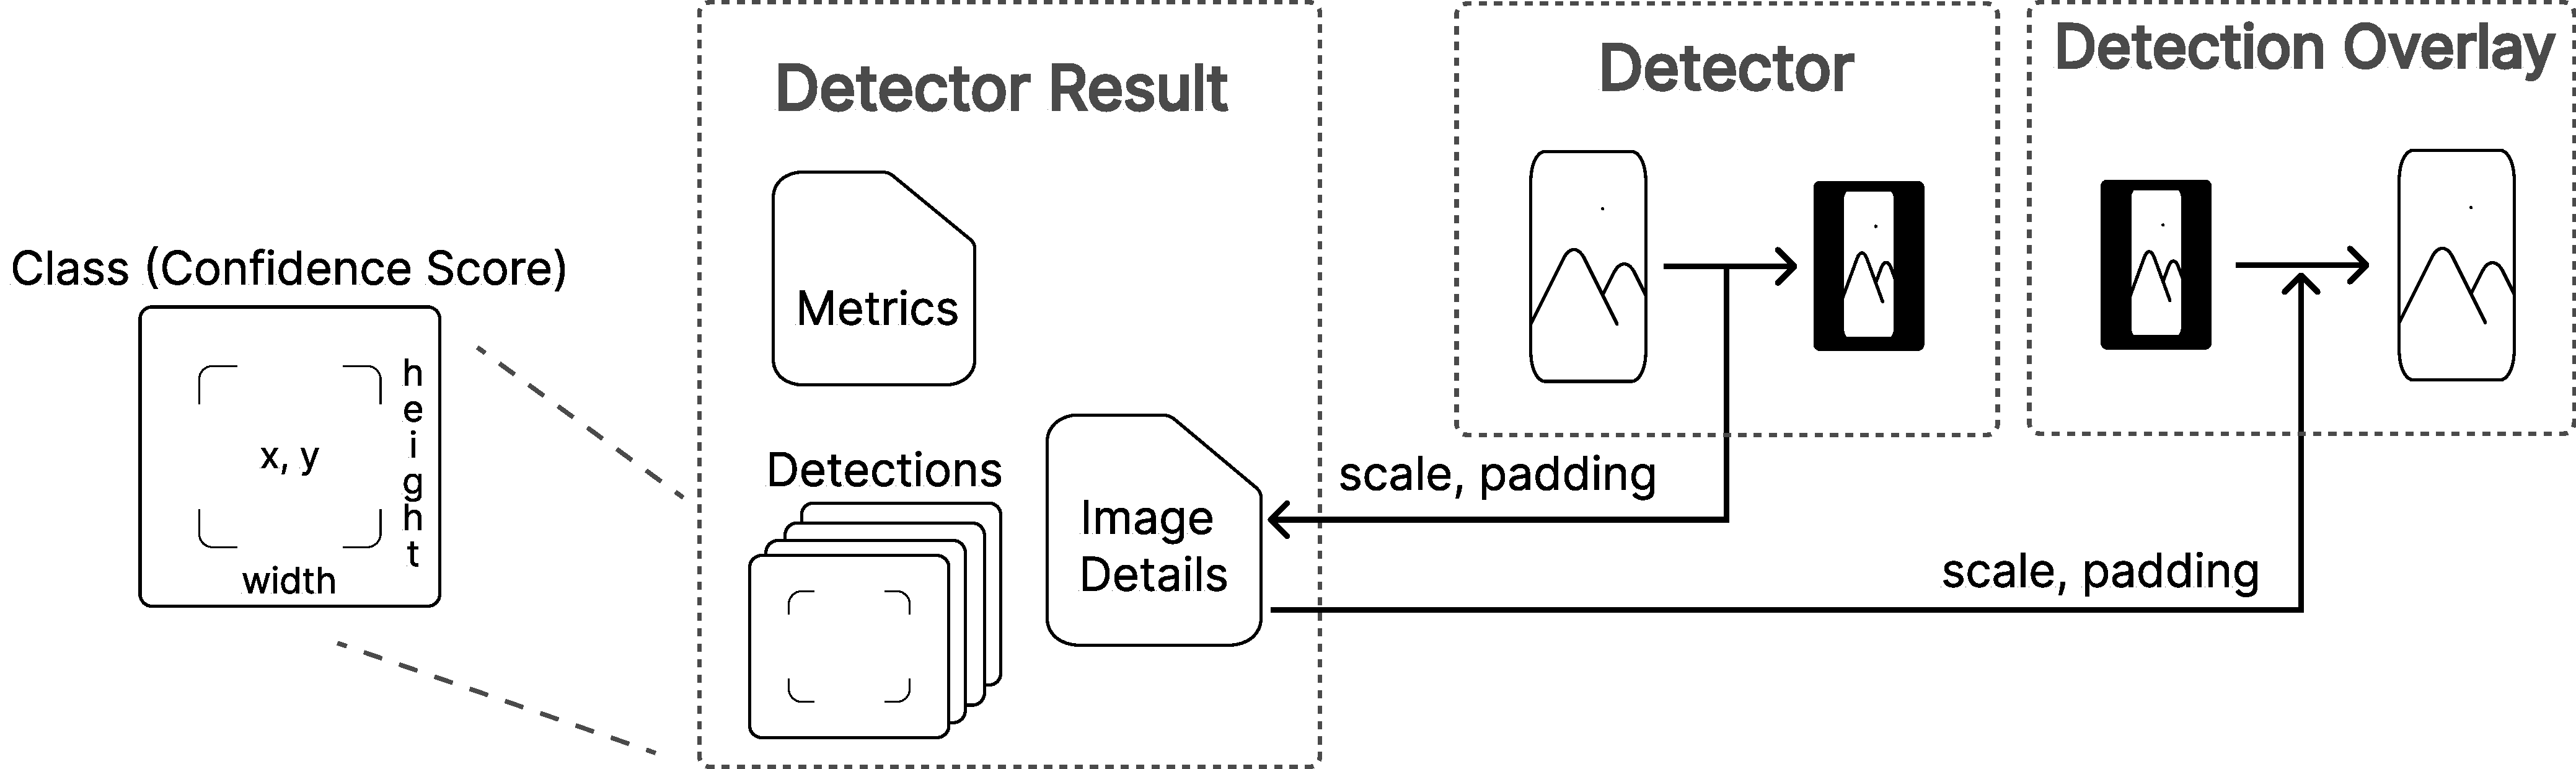
\includegraphics[width=0.95\textwidth]{obrazky-figures/data_classes.pdf}
	\caption{Scheme showing how DetectorResult is connected to other classes.}
	\label{DataClassesScheme}
\end{figure}

\label{DetectionClass}
The \texttt{Detection} data class represents a single detected object. It also contains small helper methods for converting bounding boxes to other formats using different coordinate systems, such as Kotlin's \texttt{RectF} for drawing detection or OpenCV's \texttt{Rect2d} for Non-maximum suppression. 

Class parameters are represented as follows: 

\bigskip
\begin{minipage}{\textwidth}
\begin{itemize}
  \item {X and Y represent centered coordinates of this detections bounding box in pixels.}
  \item {Width and Height values represent size in both (X and Y) dimensions in a pixels.}
  \item {Detected class for this detection.}
  \item {Confidence score of the detection.}
\end{itemize}
\end{minipage}
\bigskip


\label{ImageDetails}
The \texttt{ImageDetails} is a small data class containing changes made to the image during the preprocessing stage of object detection. These operations can be reversed in \texttt{DetectionOverlay} when displaying detections; otherwise, the detections and real world preview would not align.

\label{DetectorResult}
The \texttt{DetectorResult} is a result of \texttt{Detector} containing the list of \texttt{Detection} objects and \texttt{ImageDetails}, as well as a map of \texttt{TimerResult} and \texttt{MetricsValue} objects. These are used for performance and other metrics logging. If provided, a \texttt{MetricsOverlay} will draw these metrics onto the camera preview, providing developers with a simple debugging tool.

% ===========================================================================================

% ===========================================================================================

\section{Services}
\label{Services}
Services template classes utilizing serialization of data classes. Services contain code for loading assets, configuration files, or saving user preferences. This functionality was grouped into three services that can be used by the developers. All services require a \texttt{data class} for the template with \texttt{@Serializable} modifier. All three services work with JSON files and have a similar signature:

\begin{itemize}
    \item Application reference for loading and storing data from the device's storage.
    \item Path to the file or directory that will be loaded/saved.
    \item The \texttt{serializer} for the \texttt{data class} to which this service is tied.
    \item Character set used for reading from and writing to the file.
\end{itemize}



\subsection{ConfigService}
\label{ConfigService}
The configuration service is meant for loading and storing configuration files in JSON format. These files are stored inside the application's internal folder structure, which is beneficial for storing sensitive data, such as internal configurations that should generally not be changed using external tools. The provided \texttt{filename} parameter may point to a non-existing file; this file will be created on the next \texttt{save()} method call. Furthermore, this service requires a lambda function that returns a default value if the file is not found.

\subsection{AssetService}
\label{AssetService}
\texttt{AssetService} is used for loading JSON files from the assets folder. These files are read only. The loaded JSON file must contain a list of objects instead of a single JSON object. These objects will be loaded into memory as a map for faster look-up. Because of that, it is required to define a \texttt{keySelector}, which will be used as a key for the internal map look-ups. 

The \texttt{path} parameter of this service can be a directory, which will apply a recursive search to look for all JSON files. These will be joined to an internal map. Repetitive keys will be overridden, an error will be printed to the console, and an \texttt{onRepetitiveKeyError} callback will be invoked if it is defined.

Recursive search with multiple files provides developers with the option of separating loaded objects into groups for easier data editing; however, the JSON objects must be of the same \texttt{data class} type. Lastly, the values are \textit{lazily} evaluated on the first attempt to read them.

\subsection{StorageService}
\label{StorageService}
The storage service allows loading and saving a single JSON file, containing a list of JSON objects. Unlike the \texttt{AssetService}, it uses external storage. This location is preferred for storing logs or other data, as it can be accessed using the system file manager or when the mobile device is connected to a computer. 

Service requires \texttt{keySelector} for deciding which element of the \texttt{data class} will be used as a key for the map, used for internal storage of items.
Furthermore, the loaded file does not have to exist and can be created by the service upon saving. If the \texttt{throwOnFail} is set to \texttt{TRUE} , an exception will be thrown for the non existing file.
% ===========================================================================================

% ===========================================================================================

\section{Performance benchmark}
\texttt{PerformanceBenchmark} is a class derived from the abstract \texttt{DetectorBenchmark} class. It provides a way to log the performance of detectors. It uses a constant input image and performs multiple inference runs for the specified detector. This class provides a simple way for developers to benchmark models and export the results into the \texttt{.csv} format.

This is important, as different models and architectures for object detection may differ in performance depending on the device hardware. It is generally accepted that GPU and NPU acceleration are preferred for executing neural networks, especially object detection models. However, performance depends on hardware support and model compatibility, and some devices, especially budget ones, may not benefit from hardware acceleration. Based on the experiments performed in Chapter \ref{bangTrainingExperiments}, some models performed better on CPU than when using Android’s Neural Network API.